Per dispositivo \textit{embedded} si intende un dispositivo piccolo e compatto con consumi energetici molto contenuti. Proprio per queste caratteristiche sono usati per il \textit{deployment} di reti neurali.\\
La scelta è caduta sui dispositivi mobili. Questa decisione è stata vincolante perchè disponevamo di solo queste risorse \textit{hardware}.

\section{Conversione del modello da Keras a Tensorflow Lite}
Abbiamo convertito il modello usando \textit{Tensorflow Lite}. Il seguente codice consente di caricare il modello addestrato tramite \textit{Tensorflow} e di convertirlo nel formato .\textit{tflite} pronto per essere utilizzato su un dispositivo \textit{embedded}.
\vspace*{2ex}
\pythonexternal{./codes/tensorflowLite.py}
\noindent Il convertitore ha il compito di ottimizzare il modello riducendo le sue dimensioni e aumentando la sua velocità di esecuzione.
\section{Sviluppo applicazione Android}
\subsection{Sviluppo applicazione con Java 1.8 e Android Studio 4.1.2}
\textit{Java} è una piattaforma che consente di eseguire i programmi scritti in questo linguaggio.\\
\newline
\textit{Android Studio} è un ambiente di sviluppo integrato per lo sviluppo per la piattaforma \textit{Android}.\\
\newline
\begin{figure}[H]
	\centering
	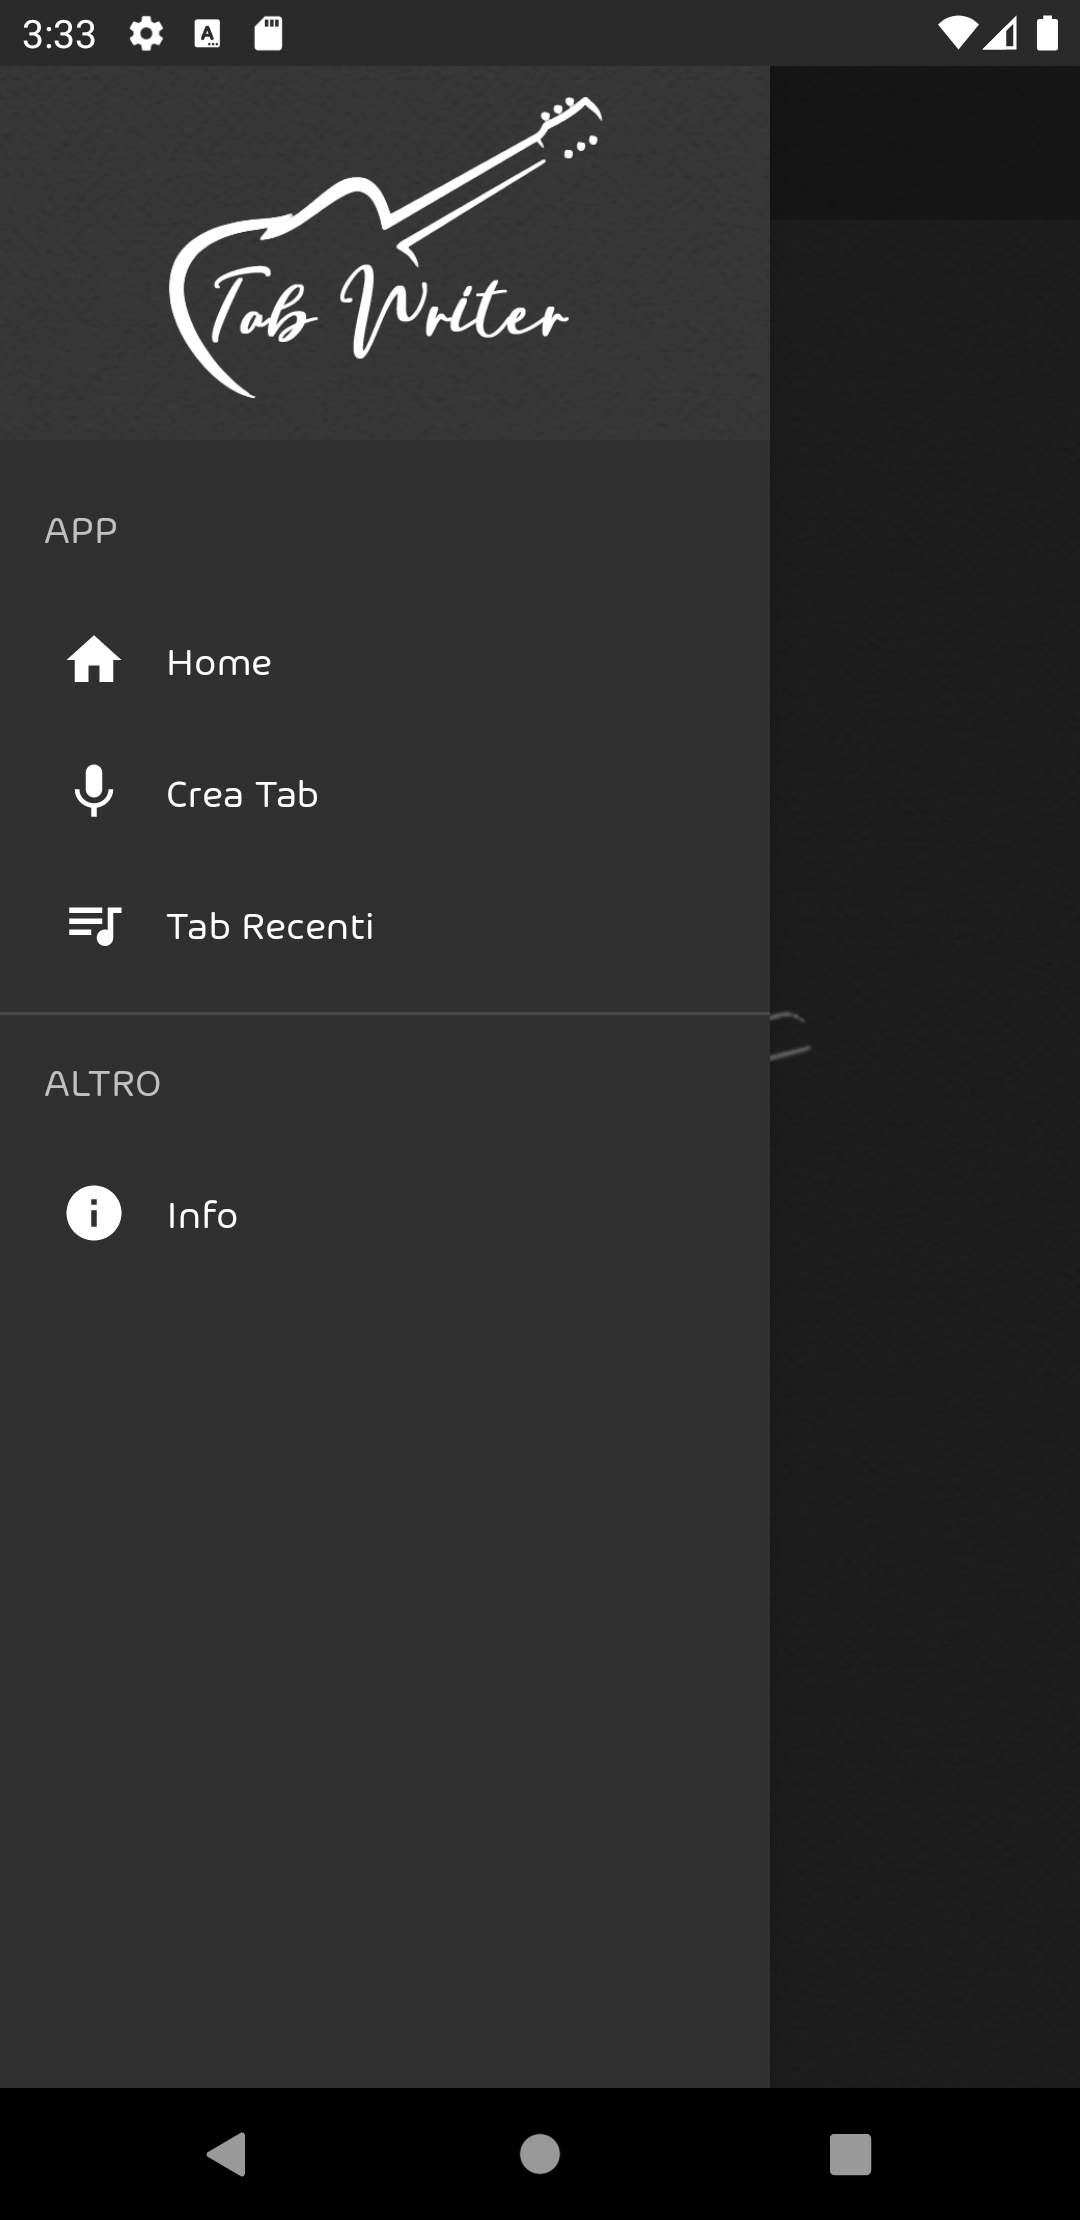
\includegraphics[scale=0.10]{./images/img17.png}
	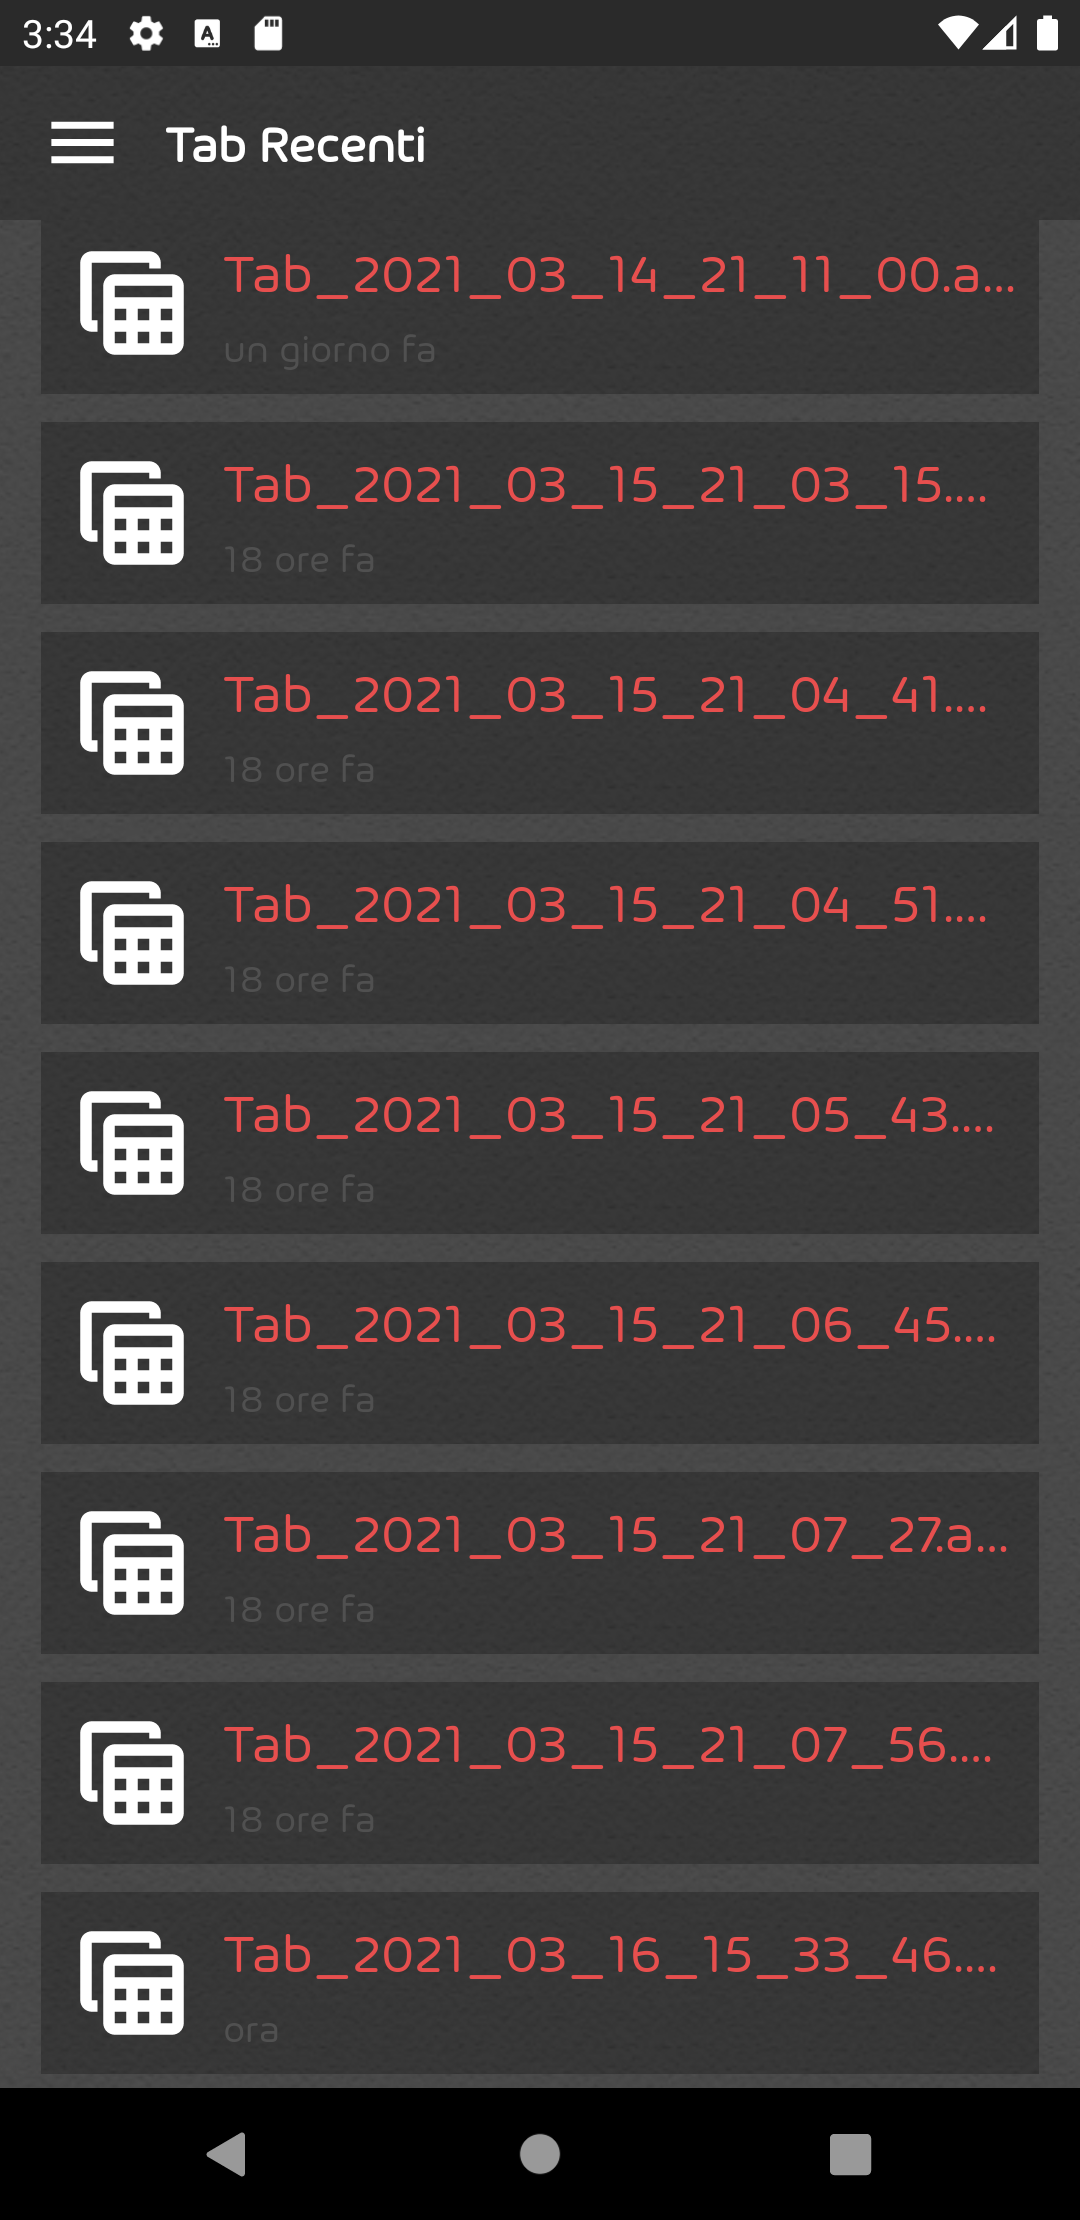
\includegraphics[scale=0.10]{./images/img20.png}
\end{figure}
\noindent Dopo aver creato le interfacce con gli elementi grafici, sia in \textit{light mode} che in \textit{dark mode}, è stato implementato un \textit{database} che tiene traccia delle \textit{tab} registrate e predette, in modo da poterle consultare anche in un secondo momento senza dover richiamare l'interprete di \textit{Tensorflow Lite}.\\
\newline
Per avviare la registrazione, basta cliccare sull'immagine centrale su cui c'è un microfono. A questo punto il cellulare registra il \textit{file} audio e per terminarla bisogna ricliccare sull'immagine.
\begin{figure}[H]
	\centering
	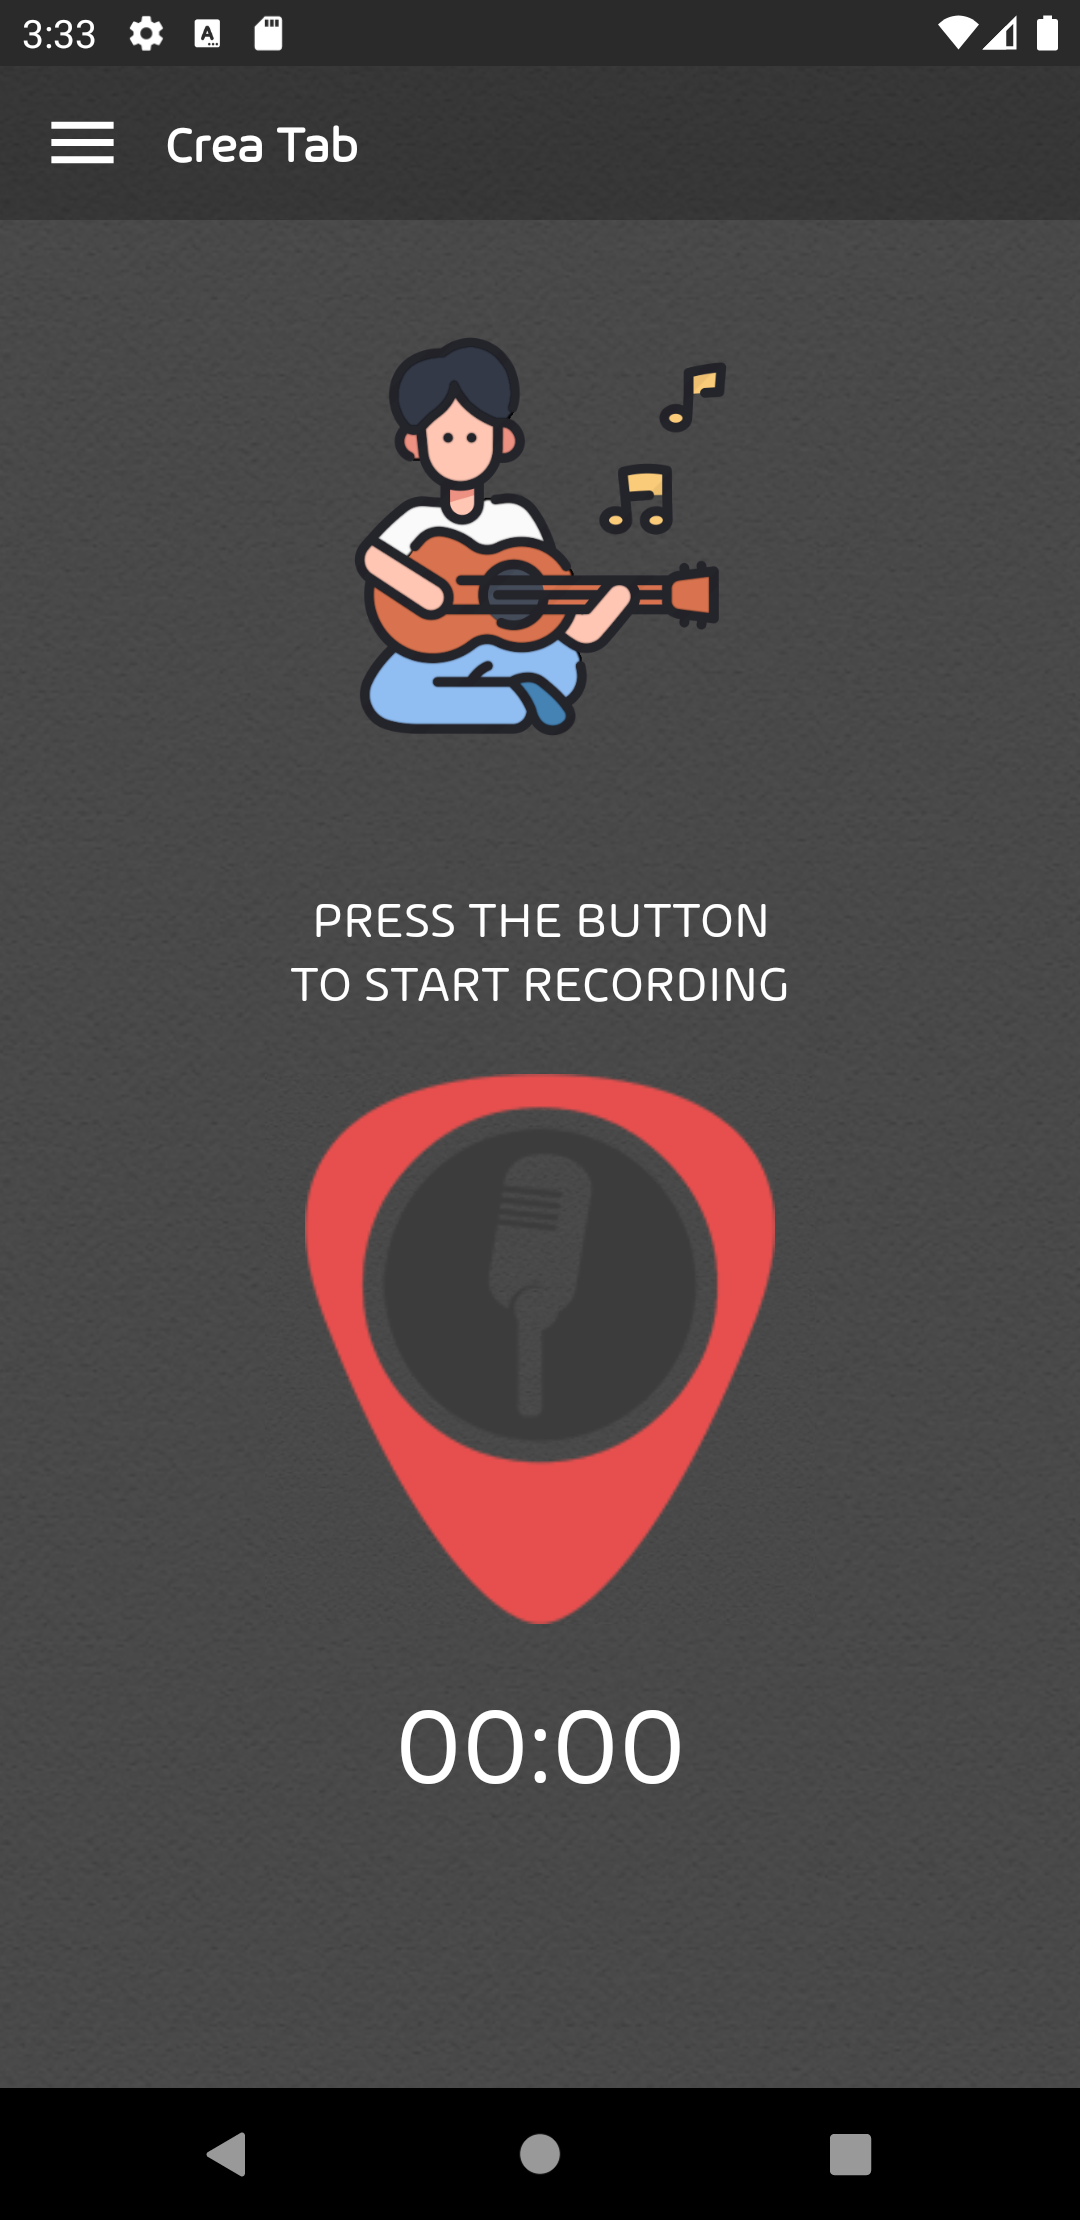
\includegraphics[scale=0.10]{./images/img18.png}
	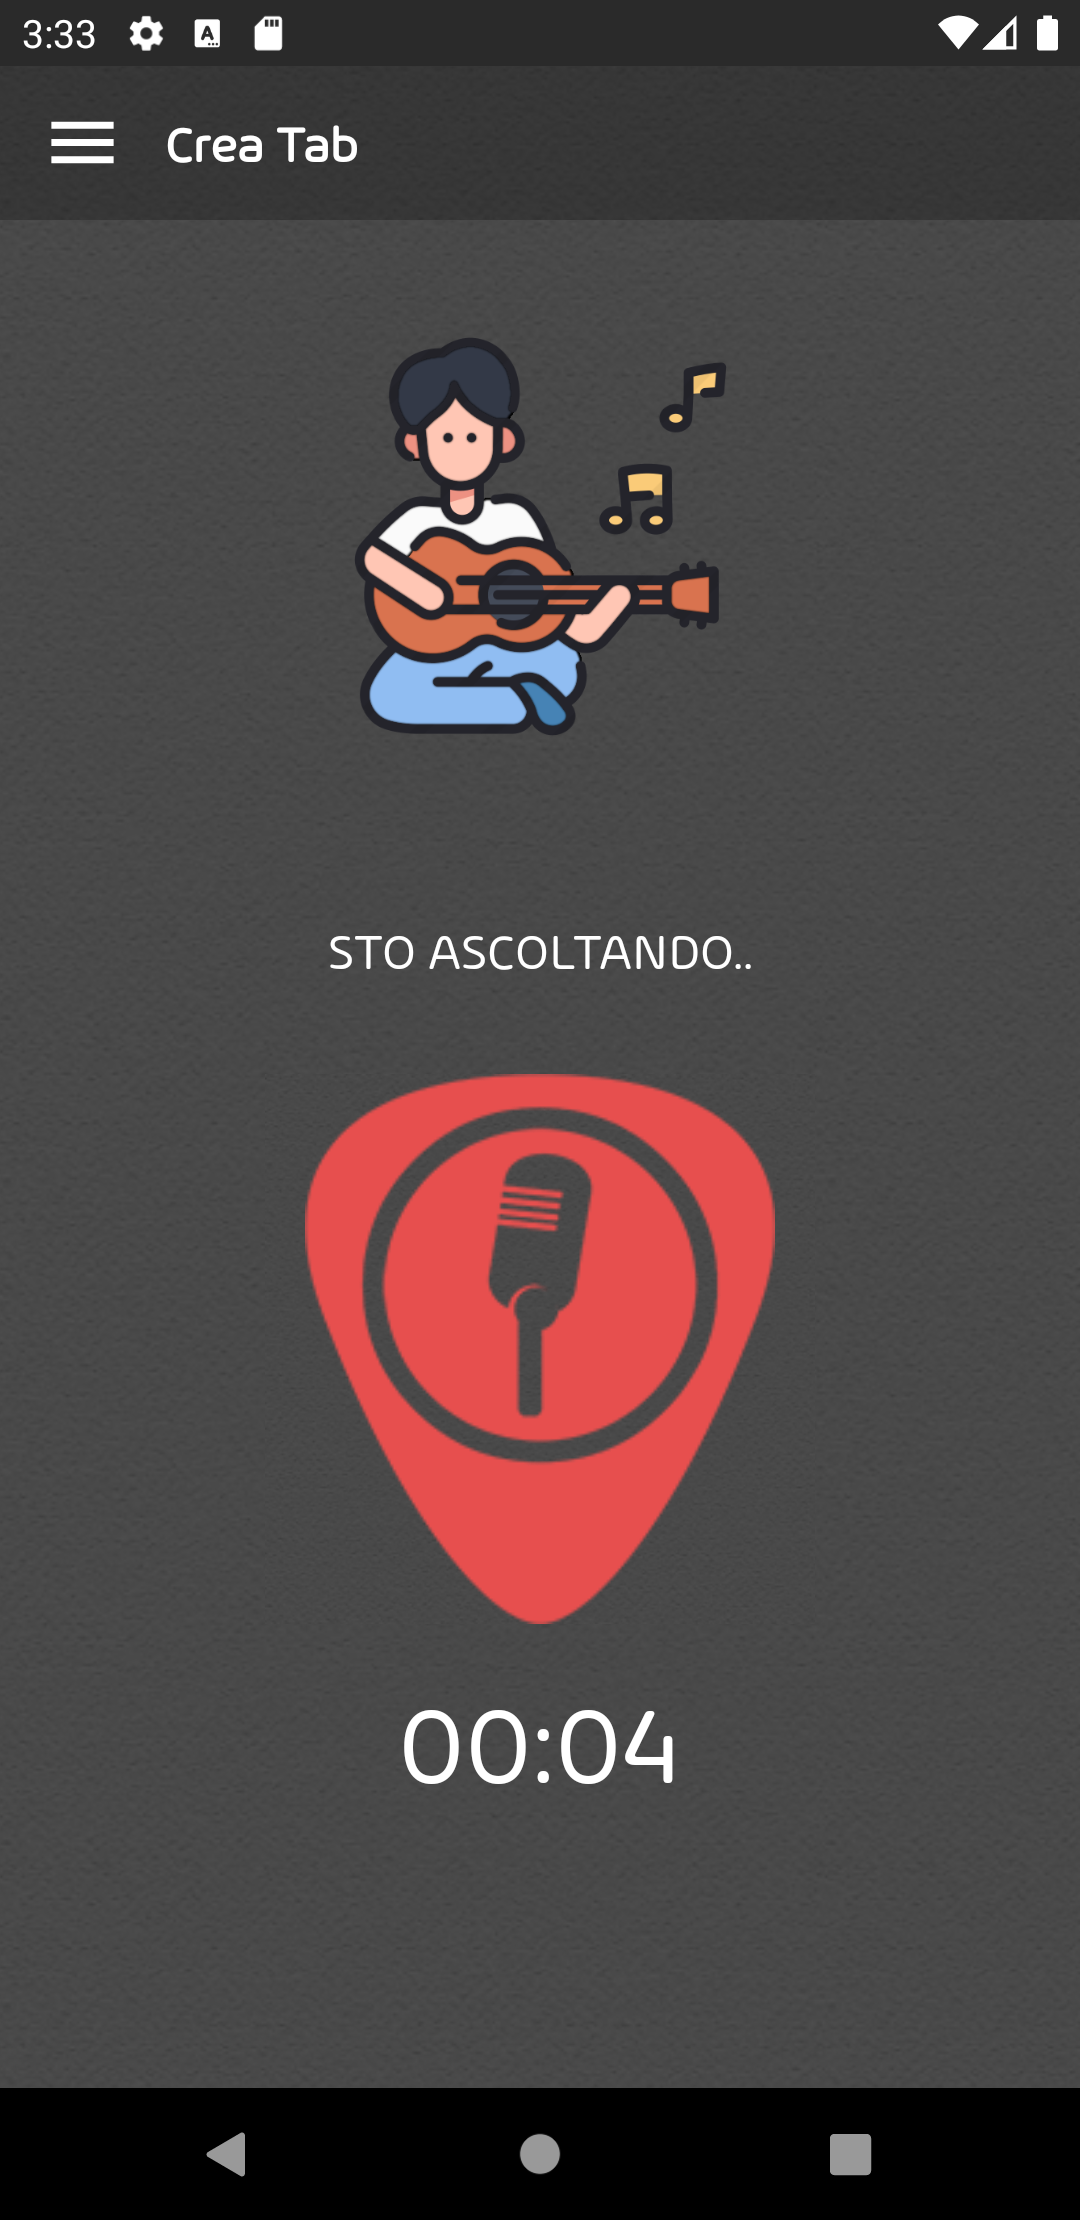
\includegraphics[scale=0.10]{./images/img22.png}
\end{figure}
\noindent A questo punto il file verrà salvato sul cellulare e convertito nel formato .\textit{wav} e grazie al modello della rete è possibile avviare la predizione. Il risultato apparirà in una nuova interfaccia:
\begin{figure}[H]
	\centering
	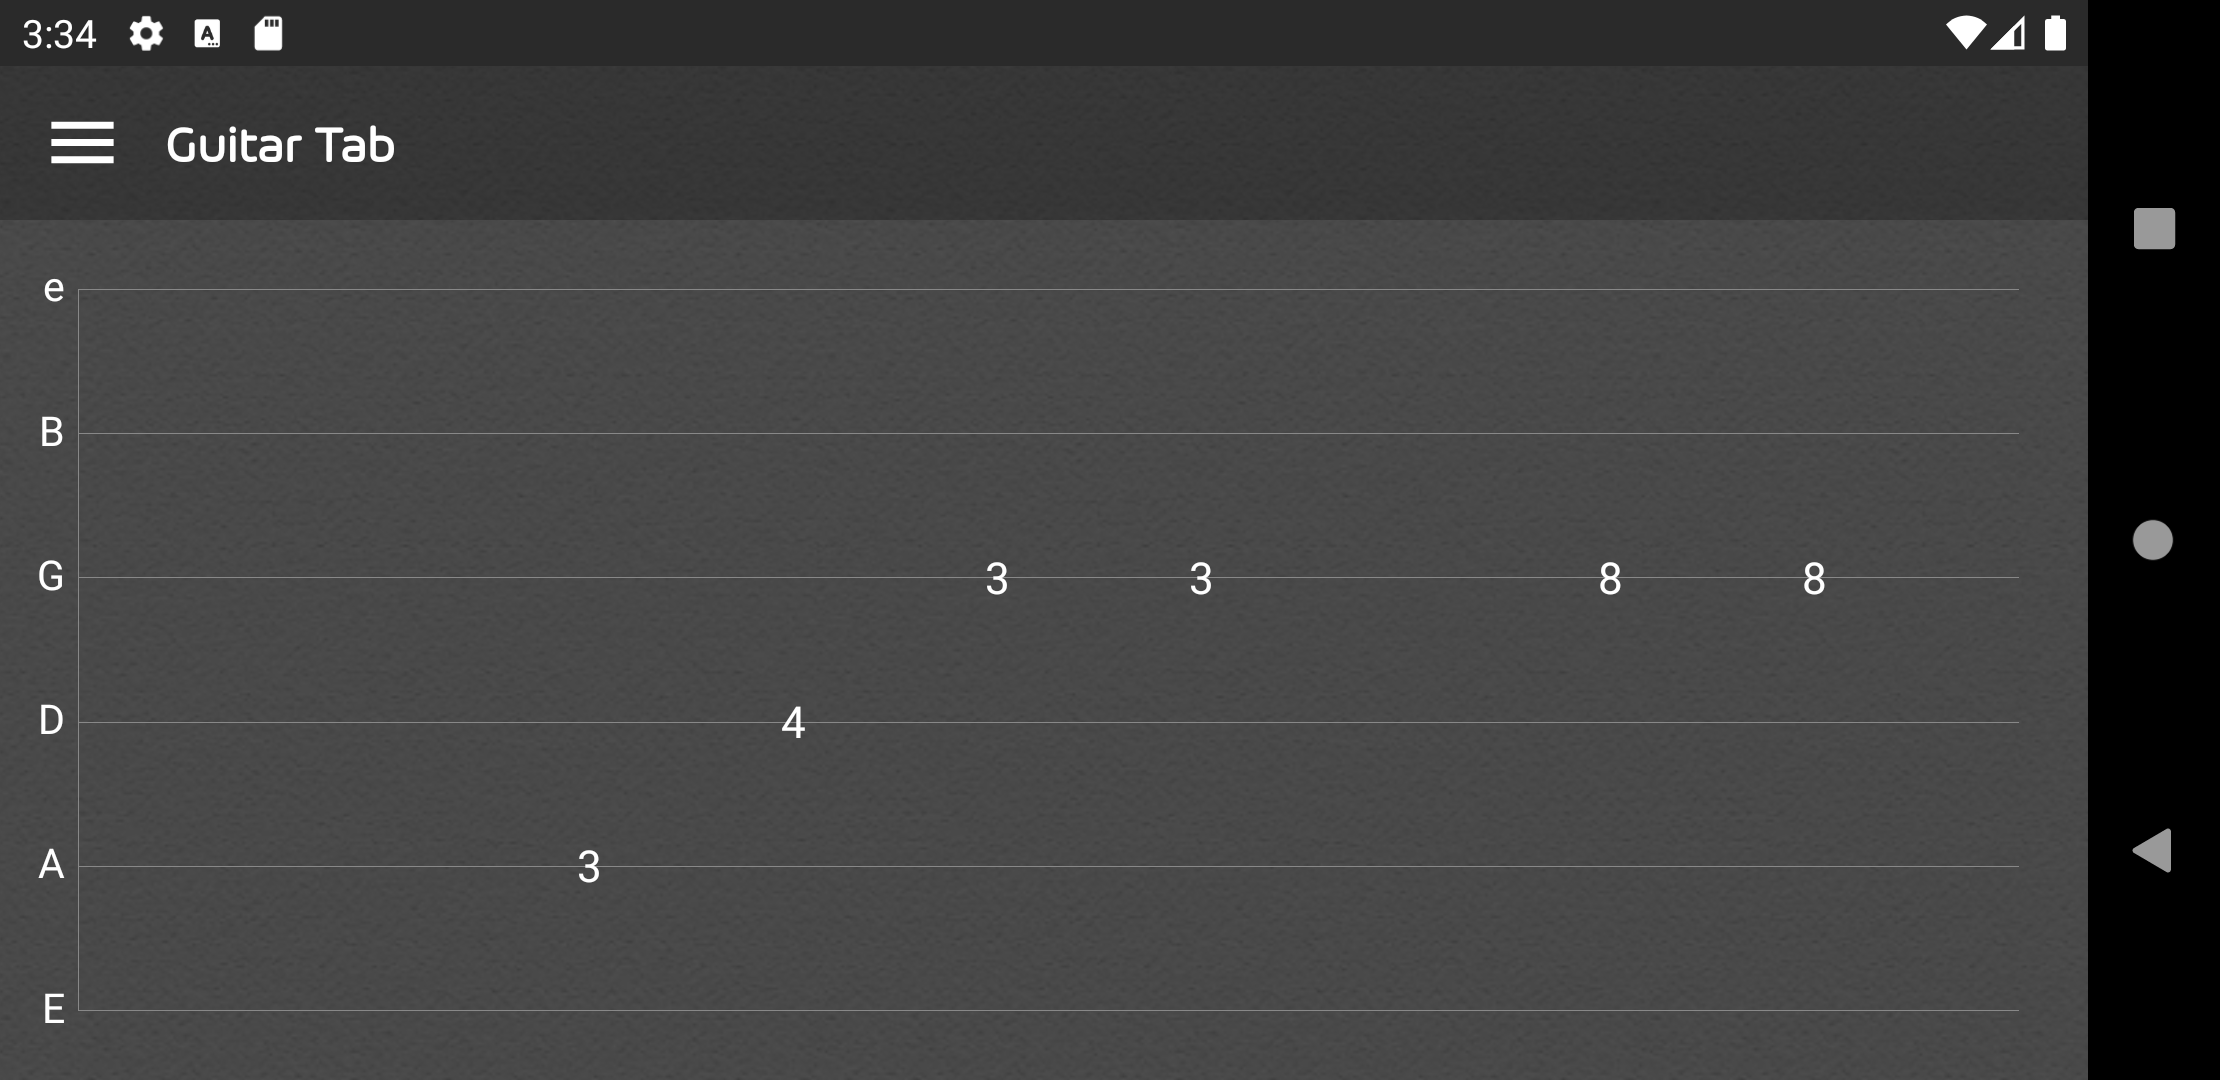
\includegraphics[scale=0.15]{./images/img19.png}
\end{figure}
\noindent \textbf{Problemi riscontrati:} putroppo non sono state trovate librerie in grado di ricavare, dal \textit{file} audio, la trasformata a Q costante come avevamo fatto su \textit{Python}.\\
\newline
%
\textbf{Soluzioni provate:}
\begin{itemize}
	\item Abbiamo pensato di utilizzare un \textit{server} che ricavi l'immagine della trasformata dall'audio registrato e la restituisca al dispositivo.\\
\end{itemize}
%
\textbf{Soluzione finale:} grazie ai ricevimenti fatti con il professore, ci è stato consigliato di usare \textit{chaquopy}, un \textit{plugin} che consente di implementare codice \textit{Python} all'interno delle applicazioni \textit{Android}.
\subsection{Pre-elaborazione dell'audio}
\textbf{Problemi riscontrati:} ricavando le immagini per ogni \textit{frame} di audio e successivamente facendo la \textit{predict} per ogni immagine, si ottenevano tante soluzioni quanti erano i \textit{frame}.\\ Per esempio, suonando il terzo tasto della quinta corda per due volte avremmo sull'interfaccia dell'applicazione una lunga serie di "3", perchè un \textit{frame} ha una durata di pochi millisecondi mentre la nota ha un \textit{range} di qualche secondo. La soluzione corretta sarebbe quella di avere solo due 3. \\
\newline
L'immagine sottostante fa vedere quanto è stato descritto:
\begin{figure}[H]
	\centering
	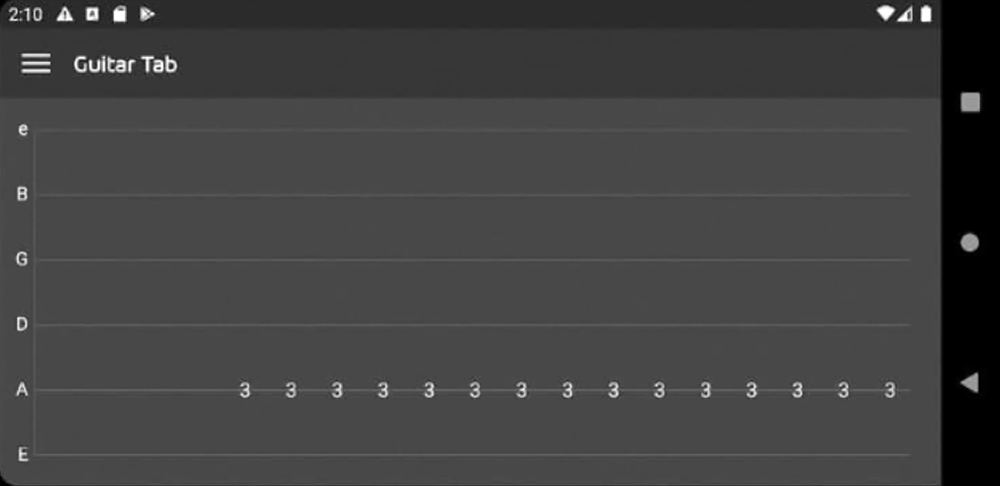
\includegraphics[scale=0.28]{./images/img25.png}
\end{figure}
\noindent \textbf{Soluzione finale:} visualizzando e analizzando lo spettrogramma, possiamo notare che quando una nota viene suonata ha un'ampiezza massima, come si può notare dal seguente grafico:
\begin{figure}[H]
	\centering
	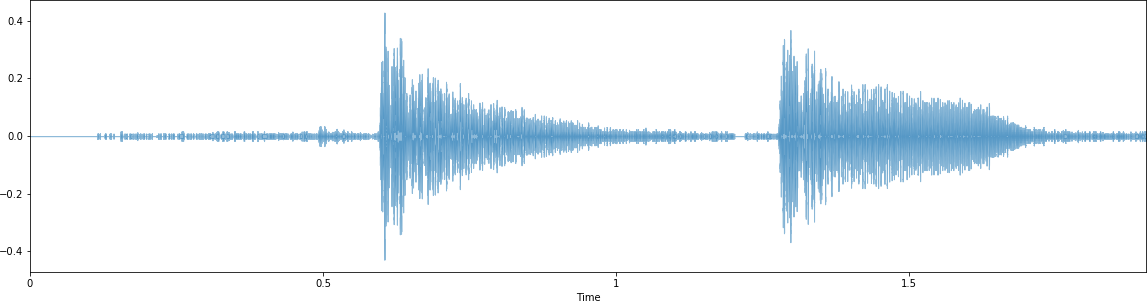
\includegraphics[scale=0.35]{./images/img26.png}
\end{figure}
\noindent Per trovare i punti, in questo caso due perchè è stata suonata due volte la stessa nota, ci viene in aiuto visualizzare l'\textit{RMS Energy} che è l'energia di un segnale. La funzione raggiunge il picco in due punti. In questo modo selezioniamo solo i \textit{frame} più significativi.
\begin{figure}[H]
	\centering
	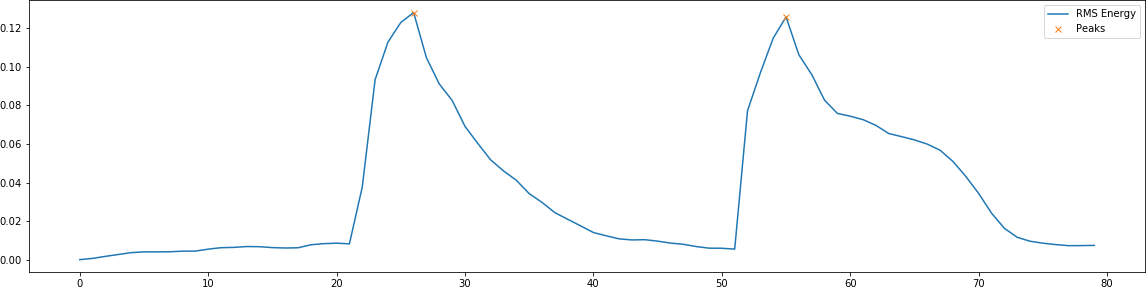
\includegraphics[scale=0.35]{./images/img27.png}
\end{figure}
\noindent Grazie alla funzione \textit{signal.find\_peaks()} della libreria \textit{scipy} troviamo tutti i massimi locali mediante un semplice confronto con i valori vicini in modo da ottenere solo i frame più significativi.
\vspace*{2ex}
\pythonexternal{./codes/preprocessing.py}
\vspace*{2ex}
Di conseguenza, vedremo solo due volte il tasto "3":
\begin{figure}[H]
	\centering
	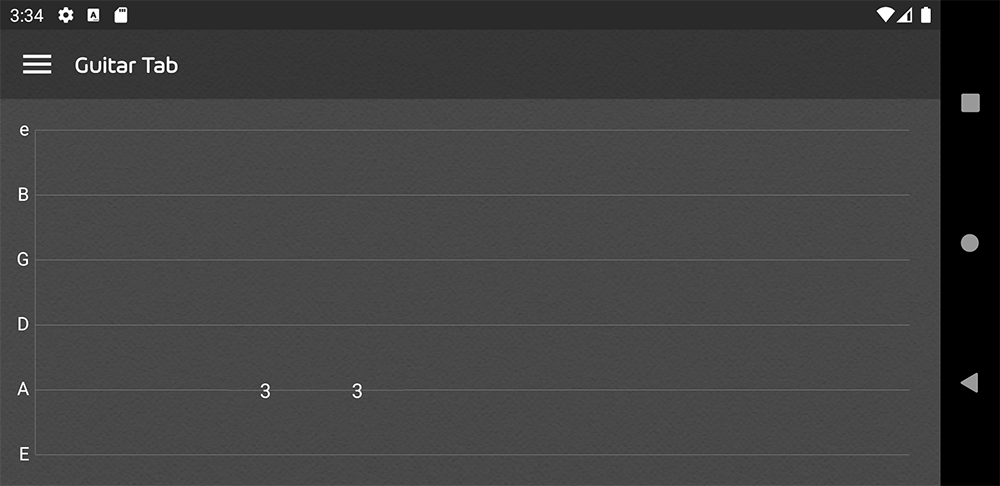
\includegraphics[scale=0.28]{./images/img24.png}
\end{figure}
\subsection{Implementazione di Tensorflow Lite}
Una volta ottenuti gli \textit{input} della rete possiamo eseguire l'inferenza con il modello. Inanzitutto rendiamo accessibile l'interprete di \textit{Tensorflow Lite}, allochiamo i tensori ed estrapoliamo dal modello rispettivamente il tipo e il formato dell'\textit{input} e dell'\textit{output}.\\ Solo i \textit{frame} più significativi verranno dati in \textit{input} all'interprete tramite la funzione \textit{interpreter.set\_tensor()}. Una volta che vengono definite le dimensione dell'\textit{input} e allocati i tensori, invochiamo l'interprete e tramite la funzione \textit{interpreter.get\_tensor()} otteniamo una copia dei valori provenienti dal tensore di \textit{output}. Infine, i risultati vengono salvati in un \textit{JSON} e conservati nel \textit{database} dell'applicazione.
\vspace*{2ex}
\pythonexternal{./codes/predict.py}
\section{Sviluppo applicazione iOS}
\subsection{Conversione del modello da Keras a CoreML}
Per poter usare il modello pre-addestrato sul cellulare abbiamo dovuto convertirlo nel formato \textit{.mlmodel} in modo da poter usare il \textit{framework Core ML}.\\
\newline
\textbf{Problemi riscontrati:} durante la conversione del modello sono apparsi diversi errori che impedivano la conversione. Gli errori sono simili a quello riportato di seguito:
\vspace*{2ex}
\textexternal{./codes/coreml.txt}
\vspace*{2ex}
\textbf{Soluzioni provate:}
\begin{itemize}
	\item Abbiamo preso spunto dal codice che si trova sul blocco di lucidi visti a lezione. Esso usa il \textit{package} \textit{tfcoreml}. Il focus dello \textit{script} è il seguente:
	\vspace*{2ex}
	\pythonexternal{./codes/coreml1.py}
	\vspace*{2ex}
	A questo punto serviva ottenere il file in formato \textit{.pb} da usare come \textit{input}. Questo file prende il nome di modello congelato. Prima di ottenerlo serve salvarci il modello che si ottiene con \textit{Tensorflow}. Esso è formato da quattro file:
	\begin{itemize}
		\item \textbf{model-ckpt.meta}: contiene il grafico completo (flusso di dati, le annotazioni per le variabili, le \textit{pipeline} di \textit{input} e altre informazioni);
     	\item \textbf{model-ckpt.data-0000-of-00001}: contiene tutti i valori delle variabili (pesi, segnaposto, gradienti, iperparametri, ecc.);
     	\item \textbf{model-ckpt.index}: ci sono tutti i metadati. È una tabella immutabile in cui ogni chiave è un nome di un tensore e il suo valore descrive i metadati di un tensore;
     	\item \textbf{checkpoint}: tutte le informazioni sul \textit{checkpoint}.
	\end{itemize}
	\vspace*{2ex}
	\pythonexternal{./codes/coreml2.py}
	\vspace*{2ex}
	\textit{estimator\_model.train()} serve a verificare che il modello esportato in precedenza sia effettivamente funzionante.\\
	\newline
	Il modello congelato ci consente di eliminare tutte le informazioni in più che vengono salvate perchè si potrebbe ricaricare quello appena salvato e l'addestramento continua da dove era stato interrotto.
	\vspace*{2ex}
	\pythonexternal{./codes/freezer.py}
	\vspace*{2ex}
	\item Uno dei nuovi tentativi si è basato sul cambio di codice per salvare il modello; abbiamo usato il seguente codice:
	\vspace*{2ex}
	\pythonexternal{./codes/coreml3.py}
	\vspace*{2ex}
	Tuttavia, i risultati non sono stati quelli sperati.
	
	\item Consultando la documentazione di \textit{coreml}, abbiamo scoperto che non sono previsti più aggiornamenti e consigliavano di usare un nuovo \textit{package}. Anche se fossimo stati in grado di convertirlo, non avremmo potuto utilizzare il modello su sistemi operativi \textit{iOS} maggiori di 12. La nuova libreria che abbiamo usato si chiama \textit{coremltools}.
	\vspace*{2ex}
	\pythonexternal{./codes/coremltools.py}
	\vspace*{2ex}
	\item Successivamente, per aumentare l'accuratezza, è stata inserita una funziona di attivazione personalizzata. Purtroppo, anche con \textit{coremltools} non siamo stati in grado di convertirlo perchè ci appariva un errore in corrispondenza del livello della nuova funzione:
	\vspace*{2ex}
	\textexternal{./codes/coremltools2.txt}
	\vspace*{2ex}
	
\end{itemize}
\textbf{Soluzione finale:} abbiamo deciso di usare \textit{Tensorflow Lite} perchè siamo riusciti a convertire il modello subito senza nessun problema.

\subsection{Sviluppo applicazione con Swift 5 e Xcode 12}
\textit{Swift} è un linguaggio di programmazione \textit{object-oriented} concepito per programmare sui sistemi operativi \textit{Apple}.\\
\newline
\textit{Xcode} è un ambiente di sviluppo integrato completamente sviluppato e mantenuto da \textit{Apple}, che consente di sviluppare \textit{software} per i sistemi \textit{macOS}, \textit{iOS}, \textit{watchOS} e \textit{tvOS}.\\
\newline
Abbiamo dovuto prendere un pò di familiarità con il nuovo linguaggio e il nuovo \textit{IDE} dato che non avevamo mai programmato nel mondo \textit{Apple}. La documentazione messa a disposizione agli sviluppatori è molto vasta e le solide basi apprese a ingegneria hanno fatto il resto.
La scelta è ricaduta direttamente sia all'ultima versione del linguaggio che dell'ambiente di sviluppo perché non avevamo vincoli sulla realizzazione dell'applicazione.\\
\newline
Le interfacce si realizzano in modo molto semplice perchè \textit{Xcode} consente di spostare gli elementi grafici con il \textit{mouse} e di posizionarli come si vuole. Tuttavia, è stata la parte che ha richiesto più tempo perchè li abbiamo dovuti configurare nel modo più adatto alle nostre esigenze.\\
\newline
E' stata prestata anche molta attenzione a rendere compatibile l'applicazione su modelli diversi. La dimensione dello schermo influisce molto sul \textit{layout} dell'applicazione. Senza le giuste modifiche è possibile che un elemento venga nascosto o spostato.
\begin{figure}[H]
	\centering
	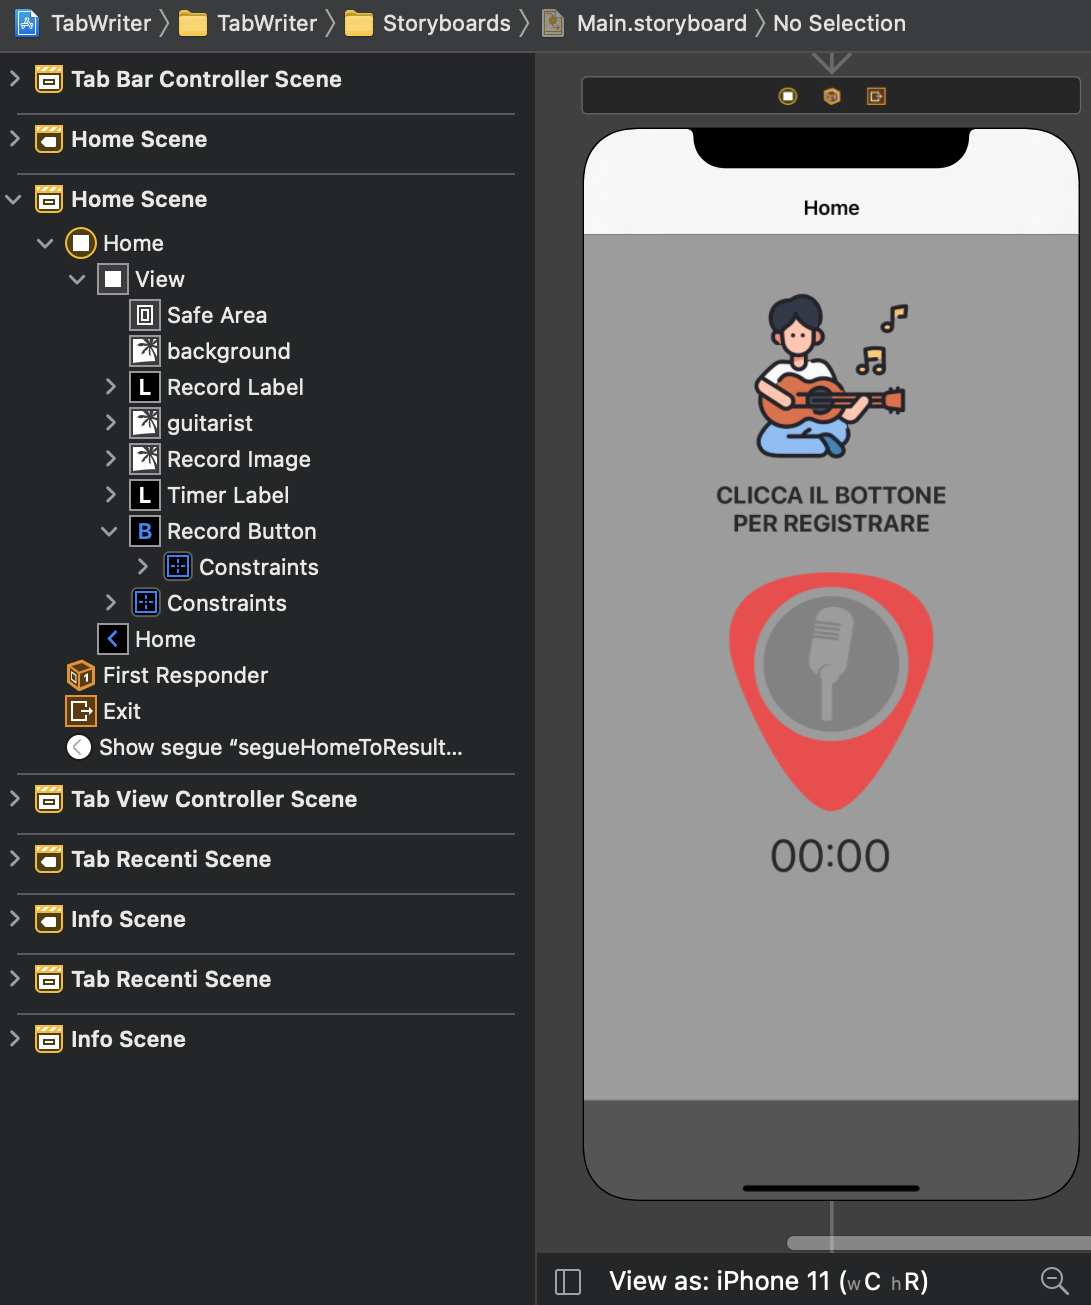
\includegraphics[scale=0.20]{./images/img2.png}
	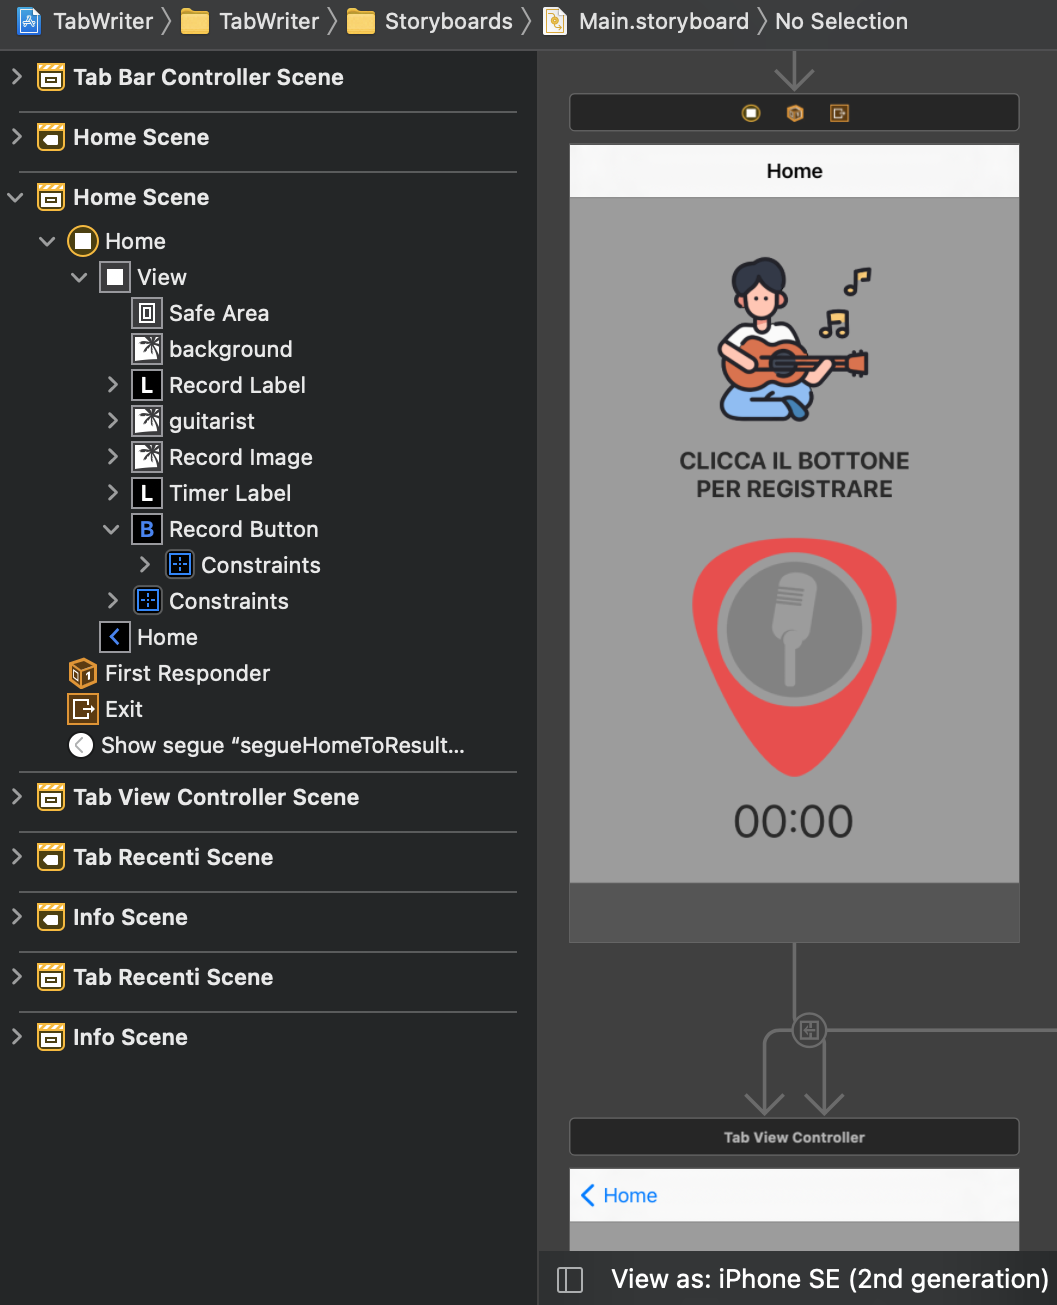
\includegraphics[scale=0.20]{./images/img3.png}
\end{figure}
\noindent Le due immagini precedenti mostrano chiaramente quello appena descritto: i due dispositivi sono diversi e le proporzioni vengono rispettate in entrambi.\\
\newline
L'applicazione che è stata realizzata da un punto di vista estetico è uguale a quella su \textit{iOS}. Cambiano solo leggeri particolari che differenziano i due mondi.\\
\newline
Inoltre, una particolare attenzione è stata dedicata anche sulla nuova modalità che sta riscontrando un grandissimo successo: la \textit{dark mode}. Dunque, sono stati presi tutti gli accorgimenti necessari per avere sia l'app compatibile con la versione chiara che con quella scura. L'immagine successiva mostra l'app in versione \textit{dark}:
\begin{figure}[H]
	\centering
	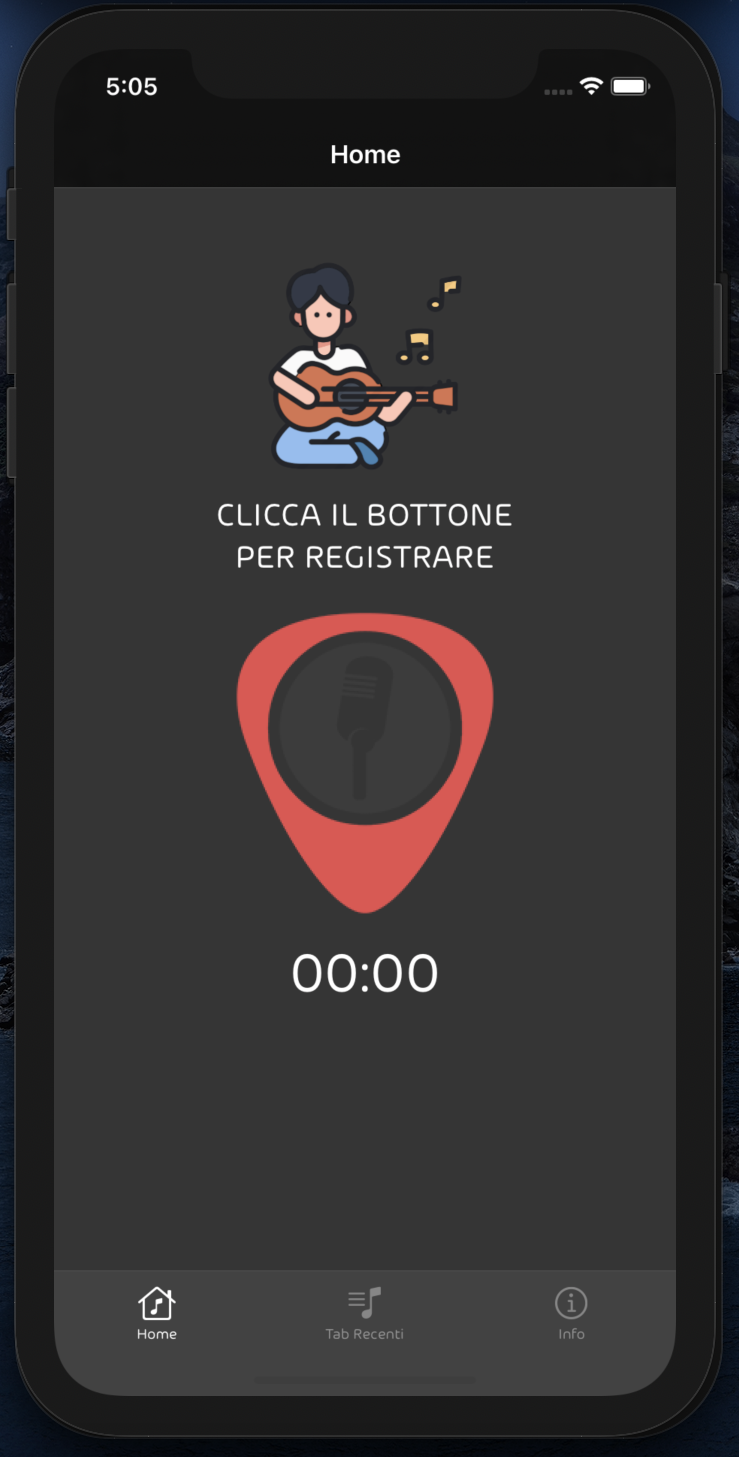
\includegraphics[scale=0.20]{./images/img10.png}
\end{figure}

\subsection{Uso di un server per l'uso della libreria librosa}
\textbf{Problemi riscontrati:} putroppo non sono state trovate librerie in grado di convertire il \textit{file} audio nella trasformata a Q costante.\\
\newline
%
\textbf{Soluzioni provate:}
\begin{itemize}
	\item Abbiamo provato ad usare la libreria \textit{PythonKit} senza successo perchè sui dispositivi \textit{iOS} manca l'interprete \textit{Python}.\\
\end{itemize}
%
\textbf{Soluzione finale:} per questo motivo ci siamo serviti di un \textit{server} che prende in ingresso la registrazione che è stata effettuata dallo \textit{smartphone} e restituisce in uscita le immagini del \textit{file} audio. Ovviamente la soluzione non è efficiente ma ai fini del progetto può andare più che bene. La predizione viene eseguita sul dispositivo e \textbf{non} sul \textit{server}.\\
\newline
Il \textit{server} è stato scritto grazie al \textit{micro-framework} \textit{Flask} scritto in \textit{Python}.
\vspace*{2ex}
\pythonexternal{./codes/flask.py}
\vspace*{2ex}
Le stesse operazioni descritte nel \textit{paragrafo 4.2.2} vengono eseguite dal \textit{server} che infatti ritorna solo i \textit{frame} più significativi.
\subsection{Implementazione di Tensorflow Lite}
Per utilizzare il nostro modello \textit{TensorFlow Lite} all'interno dell'applicazione, abbiamo dovuto prima configurare il progetto usando la libreria \textit{Firebase} e poi istanziato l'interprete per poterlo caricare. Nel seguente codice l'interprete viene istanziato grazie a \textit{Interpreter()}.
\vspace*{2ex}
\swiftexternal{./codes/tensorflowLiteIos1.swift}
\vspace*{2ex}
\noindent Per eseguire l'inferenza è necessario effettuare delle trasformazioni sui dati che sono obbligatorie per poterli dare in ingresso al modello. L'\textit{input} della rete deve essere un oggetto \textit{Data} al cui interno sono presenti i dati dell'\textit{array}contenente le immagini del \textit{file} audio (\textit{inputImages}).\\
A questo punto si allocano i tensori, si inserisce l'\textit{input} nella rete e si chiama il metodo \textit{invoke()}.
È possibile ottenere il tensore di \textit{output} chiamando il metodo \textit{output(at:)} e gli elementi ottenuti dalla predizione tramite \textit{output.data.copyBytes}. Inoltre, si può notare che ci sono due cicli: quello esterno serve per leggersi tutte le immagini della registrazione mentre il secondo funge da \textit{check} per verificare che l'immagine corrisponda a uno di quei picchi di cui abbiamo parlato in precedenza.
\vspace*{2ex}
\swiftexternal{./codes/tensorflowLiteIos2.swift}
\subsection{Installazione su dispositivo fisico}
L'applicazione è stata installata non solo sul simulatore ma anche sul dispositivo fisico. Lo \textit{smartphone} è un \textit{Iphone 11} con sistema operativo \textit{iOS} 14.1.
\begin{figure}[H]
	\centering
	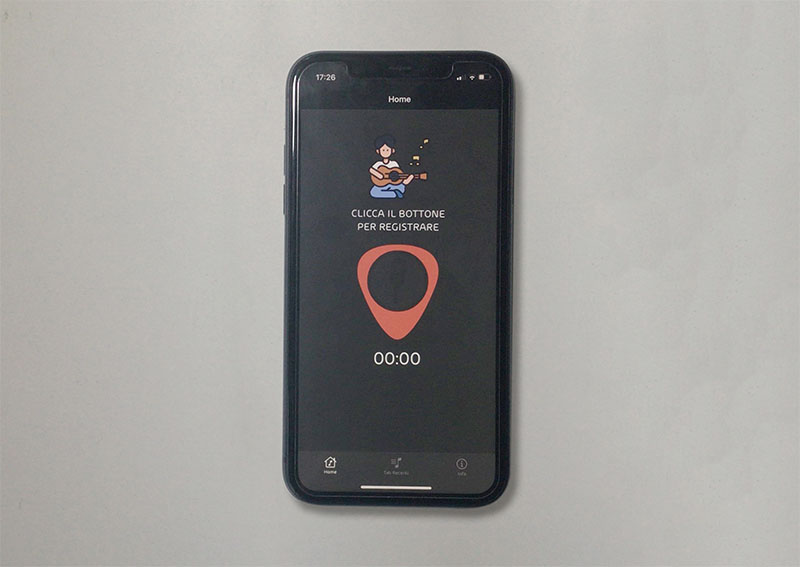
\includegraphics[scale=0.40]{./images/img21.jpg}
\end{figure}